%% SECTION HEADER ////////////////////////////////////////////////////////////////////////////////
\section{Synthetic dataset acquisition}
\label{sec41}
%%%%%%%%%%%%%%%%%%%%%%%%%%%%%%%%%%%%%%%%%%%%%%%%%%%%%
The essential part of this work was in generating a synthetic dataset of a full wavefield of propagating Lamb waves in a plate made of CFRP.
Therefore, in this work, a numerical dataset of propagating waves in carbon fibre reinforced composite plates was computed by using the parallel implementation of the time domain spectral element method~\cite{Kudela2020}.

The dataset resembles the particle velocity measurements at the bottom surface of the plate acquired by the SLDV in the transverse direction as a response to the piezoelectric (PZT) excitation placed at the centre of the plate. 
The input signal was a five-cycle Hann window modulated sinusoidal tone burst. 
The carrier frequency was assumed to be 50 kHz. 
The total wave propagation time was set to 0.75 ms so that the guided wave could propagate to the plate edges and back to the actuator twice.
The number of time integration steps was 150000, which was selected for the stability of the central difference scheme.

The material was a typical cross-ply CFRP laminate. 
The stacking sequence [0/90]\(_4\) was used in the model. 
The properties of a single ply were as follows [GPa]:
\(C_{11} = 52.55, \, C_{12} = 6.51, \, C_{22} = 51.83, C_{44} = 2.93, C_{55} = 2.92, C_{66} = 3.81\). 
The assumed mass density was 1522.4 kg/m\textsuperscript{3}.
These properties were selected so that wavefront patterns and wavelengths simulated numerically are similar to the wavefields measured by the SLDV on CFRP specimens used later on for testing the developed methods for delamination identification.
The shortest wavelength of the propagating A0 Lamb wave mode was 21.2 mm for numerical simulations and 19.5 mm for experimental measurements, respectively.

For each case, single delamination was modelled by using the method of splitting nodes between appropriate spectral elements. 
It was assumed that the composite laminate is made of eight layers of a total thickness of 3.9 mm.
The delamination was modelled between the third and fourth layer (see Fig.~\ref{fig:plate_setup} for details).
It should be noted that Fig.~\ref{fig:plate_setup} shows an exaggerated cross-section through the delamination. 
Zero-volume delamination was assumed in the model. 
Delamination spatial location was selected randomly so that the interaction of guided waves with delamination is different for each case.
It includes cases when delamination is located at the edge of the plate, which is the most difficult to identify by signal processing methods.
\begin{figure}
	\centering
	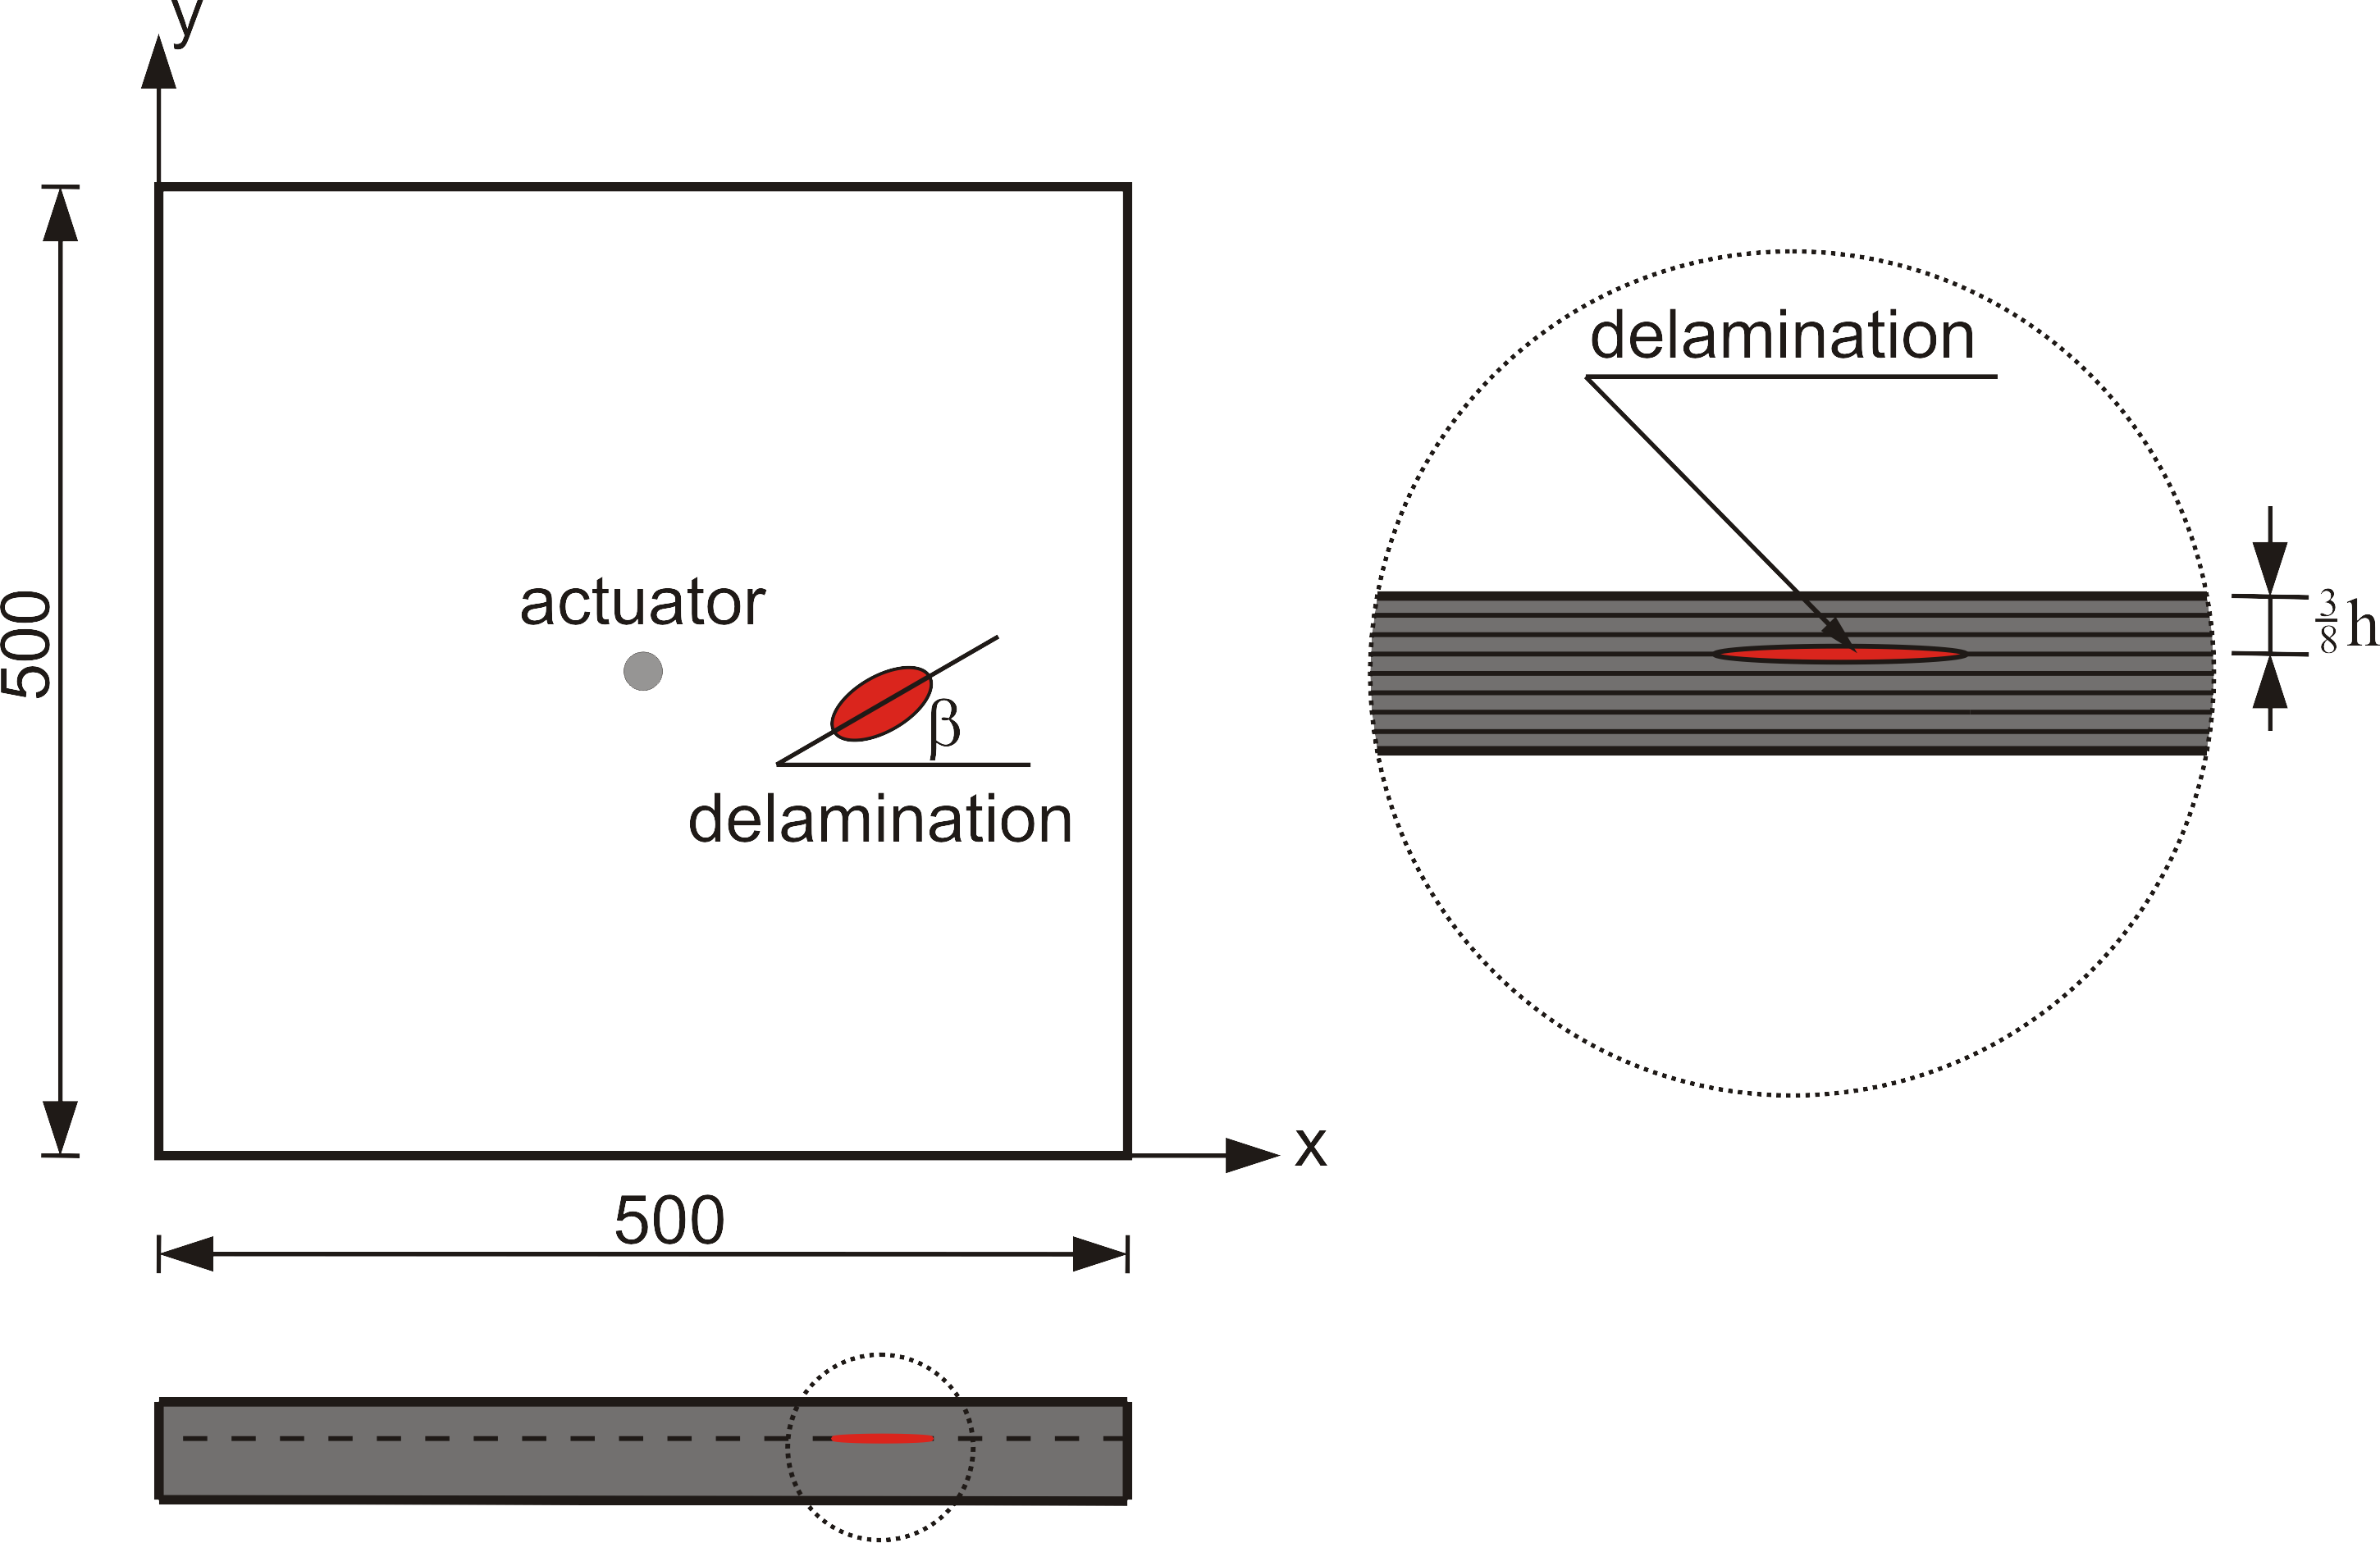
\includegraphics[scale=1]{Figures/Chapter_4/plate_delam_arrangement_MSSP.PNG}
	\caption{Setup for computing Lamb wave interactions with delamination.}
	\label{fig:plate_setup}
\end{figure}
Additionally, the size of the delamination of elliptic shape was randomly simulated by selecting the size of the ellipse minor and major axes.
Furthermore, the angle between the delamination major axis and the horizontal axis was randomly selected.
In summary, the following random parameters were simulated in each case:
\begin{itemize}
	\item delamination geometrical size	(ellipse minor and major axis randomly selected from the interval \(\left[10 \, \textrm{mm}, 40\, \textrm{mm}\right]\)),
	\item delamination angle (randomly selected from the interval \( \left[ 0^{\circ}, 180^{\circ} \right]\)),
	\item coordinates of the centre of delamination (randomly selected from the interval \(\left[0\, \textrm{mm}, 250\, \textrm{mm} -\delta \right]\) and \( \left[250\, \textrm{mm}+\delta, 500\, \textrm{mm} \right] \), where \(\delta = 10\, \textrm{mm}\)).
\end{itemize}
These parameters are defined in Fig.~\ref{fig:random_delaminations}, which shows exemplary random delamination locations, sizes, and shapes for Lamb wave propagation modeling.
And it is important to note that the numerical cases include delaminations at the edges and the corners of the plate and corners.
\begin{figure}[!h]
	\centering
	\includegraphics[scale=0.8]{Figures/Chapter_4/figure1.png}
	\caption{Exemplary locations, sizes and shapes of random delaminations used for Lamb wave propagation modeling.}
	\label{fig:random_delaminations}
\end{figure}

It resulted in random spatial placement of delaminations. The plate with overlayed 475 delamination cases is shown in Fig.~\ref{fig:random_delam}.
\begin{figure}
	\centering
	\includegraphics[scale=1.25]{Figures/Chapter_4/dataset2_labels_ellipses.png}
	\caption{The plate with 475 cases of random delaminations.}
	\label{fig:random_delam}
\end{figure}

The output from the top and bottom surfaces of the plate in the form of particle velocities at the nodes of spectral elements were interpolated on the uniform grid of 500\(\times\)500 points by using shape functions of elements (see~\cite{Kudela2020} for more details).
It essentially resembles measurements acquired by SLDV in the transverse direction (perpendicular to the plate surface).
An example of the simulated full wavefield data on the top and bottom surfaces is presented in Fig.~\ref{fig:wavefield}.
It should be noted that stronger wave entrapment at delamination can be observed for the case of the wavefield at the top surface.
It is because the delamination within the cross-section is located closer to the top surface.
It makes it easier to detect delamination by processing wavefields at the top surface.
It is better visible if the root mean square (RMS) according to Eq.~(\ref{eq:rms}) is applied to the wavefield.
The result of this operation is presented in Fig.~\ref{fig:rms}.
Based on the image analysis, the shape of the delamination can be easier to discern for the top case.
\begin{figure} [h!]
	\centering
	\begin{subfigure}[b]{0.32\textwidth}
		\centering
		\includegraphics[scale=1]{Figures/Chapter_4/96_flat_shell_Vz_1_500x500top.png}
		\caption{\(t=0.141\) ms}
		\label{fig:frame96top}
	\end{subfigure}
	\hfill
	\begin{subfigure}[b]{0.32\textwidth}
		\centering
		\includegraphics[scale=1]{Figures/Chapter_4/128_flat_shell_Vz_1_500x500top.png}
		\caption{\(t=0.188\) ms}
		\label{fig:frame128top}
	\end{subfigure}
	\hfill
	\begin{subfigure}[b]{0.32\textwidth}
		\centering
		\includegraphics[scale=1]{Figures/Chapter_4/164_flat_shell_Vz_1_500x500top.png}
		\caption{\(t=0.240\) ms}
		\label{fig:frame164top}
	\end{subfigure}	
	\hfill
	\begin{subfigure}[b]{0.32\textwidth}
		\centering
		\includegraphics[scale=1]{Figures/Chapter_4/96_flat_shell_Vz_1_500x500bottom.png}
		\caption{\(t=0.141\) ms}
		\label{fig:frame96bottom}
	\end{subfigure}
	\hfill
	\begin{subfigure}[b]{0.32\textwidth}
		\centering
		\includegraphics[scale=1]{Figures/Chapter_4/128_flat_shell_Vz_1_500x500bottom.png}
		\caption{\(t=0.188\) ms}
		\label{fig:frame128bottom}
	\end{subfigure}
	\hfill
	\begin{subfigure}[b]{0.32\textwidth}
		\centering
		\includegraphics[scale=1]{Figures/Chapter_4/164_flat_shell_Vz_1_500x500bottom.png}
		\caption{\(t=0.240\) ms}
		\label{fig:frame164bottom}
	\end{subfigure}
	
	\caption{Full wavefield at the top surface (a)--(c) and the bottom surface (d)--(f), respectively, at selected time instances showing the interaction of guided waves with delamination.}
	\label{fig:wavefield}
\end{figure} 

\begin{figure} [h!]
	\centering
	\begin{subfigure}[b]{0.47\textwidth}
		\centering
		\includegraphics[scale=1]{Figures/Chapter_4/RMS_flat_shell_Vz_1_500x500top.png}
		\caption{top}
		\label{fig:rmstop}
	\end{subfigure}
	\hfill
	\begin{subfigure}[b]{0.47\textwidth}
		\centering
		\includegraphics[scale=1]{Figures/Chapter_4/RMS_flat_shell_Vz_1_500x500bottom.png}
		\caption{bottom}
		\label{fig:rmsbottom}
	\end{subfigure}
	\caption{RMS of the full wavefield from the top surface of the plate (a) and the bottom surface of the plate (b).}
	\label{fig:rms}
\end{figure} 
\newpage